%%% lecture 08 %%%
\documentclass{beamer}
\usepackage[utf8]{inputenc}
\usepackage{algorithm2e, amsmath, amssymb, amsfonts, graphicx, hyperref}
% allow section.equation numbering
\numberwithin{equation}{section}
% use boadilla theme
\usetheme{Boadilla}
% remove navigation symbols
\usenavigationsymbolstemplate{}
% get numbered figure captions
\setbeamertemplate{caption}[numbered]
% changes itemize to circle + other things
\useoutertheme{split}
\useinnertheme{circles}

% command for the title string. change for each lecture
\newcommand{\lecturetitle}{Support Vector Machines}
% allow automatic alert-highlighted references and hyperlinks
\newcommand{\aref}[1]{\alert{\ref{#1}}}
\newcommand{\ahref}[2]{\href{#1}{\alert{#2}}}
% title page stuff. brackets content displayed in footer bar
\title[\lecturetitle]{\lecturetitle}
% metadata. content in brackets is displayed in footer bar
\author[Derek Huang (BAC Advanced Team)]{Derek Huang}
\institute{BAC Advanced Team}
\date{October 12, 2021}

% change "ball" bullet to numbered bullet and section title for section
\setbeamertemplate{section in toc}{\inserttocsectionnumber.~\inserttocsection}
% change ball to gray square (copied from stackoverflow; \par needed for break)
\setbeamertemplate{subsection in toc}{        
    \hspace{1.2em}{\color{gray}\rule[0.3ex]{3pt}{3pt}}~\inserttocsubsection\par
}
% use default enumeration scheme
\setbeamertemplate{enumerate items}[default]
% required line that fixes the problem of \mathbf, \bf not working in beamer
% for later (post-2019) TeX Live installations. see the issue on GitHub:
% https://github.com/josephwright/beamer/issues/630
\DeclareFontShape{OT1}{cmss}{b}{n}{<->ssub * cmss/bx/n}{}

\begin{document}

% title slide
\begin{frame}
    \titlepage
    \centering
    % relative path may need to be updated depending on .tex file location
    
\includegraphics[scale=0.1]{../bac_logo1.png}
\end{frame}

% table of contents slide
\begin{frame}{Overview}
    \tableofcontents
\end{frame}


\section{Separating hyperplanes}

\subsection{Hyperplanes and halfspaces}

\begin{frame}{Motivation}
    \begin{itemize}
        \item
        We saw that logistic regression, LDA/QDA, and na\"{i}ve Bayes
        provide probabilistic models of [class-]conditional distributions.

        \item
        Suppose we have disjoint convex sets $ A, B \subset \mathbb{R}^d $.
        There are several ways to draw a distribution-free ``line''
        (hyperplane) between them.

        \item
        Intuitively, the optimal hyperplane is furthest away from both
        $ A, B $. How can solve the resulting optimization problem?

        \item
        How do we define ``furthest away'' in this context?
    \end{itemize}
\end{frame}

\begin{frame}{Hyperplanes and halfspaces}
    \begin{itemize}
        \item
        \textit{Definition.} A \textit{hyperplane} in $ \mathbb{R}^d $ with
        \textit{normal vector} $ \mathbf{a} \in \mathbb{R}^d $ is the affine
        set
        $ \{\mathbf{x} \in \mathbb{R}^d : \mathbf{a}^\top\mathbf{x} = b \} $,
        where $ \mathbf{a} \ne \mathbf{0} $, $ b \in \mathbb{R} $
        \cite{bv_convex_opt}.

        \item
        A hyperplane is the solution set for a nontrivial linear equation with
        a \textit{normal vector} $ \mathbf{a} $, which in 2D is orthogonal
        to the plane.

        \begin{figure}
            \centering
            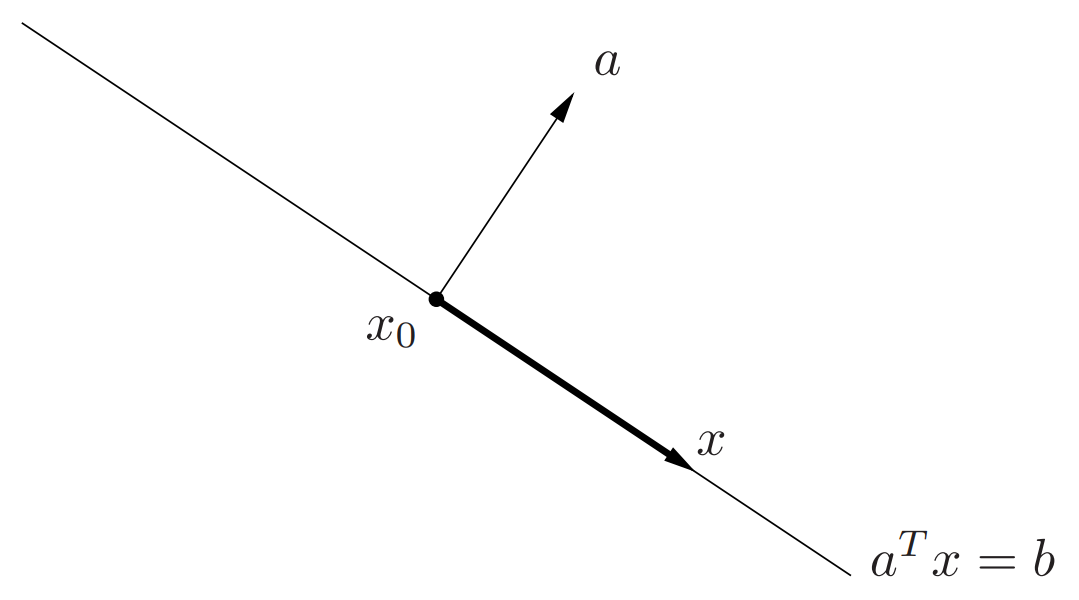
\includegraphics[scale=0.2]{hyperplane.png}
            \vspace{-5 pt}
            \caption{
                A hyperplane with normal vector $ \mathbf{a} \in
                \mathbb{R}^2 $. Note $ \mathbf{a}^\top(\mathbf{x} -
                \mathbf{x}_0) = 0 $\footnote{
                    Figure 2.6 from Boyd and Vandenberghe's
                    \textit{Convex Optimization}.                
                }.
            }
            \label{fig:hyperplane}
            \vspace{-5 pt}
        \end{figure}

        \item
        As seen in Figure \aref{fig:hyperplane}, for hyperplane
        $ L \triangleq \{\mathbf{x} \in \mathbb{R}^d :
        \mathbf{a}^\top\mathbf{x} = b \} $,
        $ \forall \mathbf{x}, \mathbf{y} \in L $,
        $ \mathbf{a}^\top(\mathbf{x} - \mathbf{y}) = 0 \Rightarrow \mathbf{a} $
        is orthogonal to vectors parallel to $ L $.
    \end{itemize}

    % spacing for footnote
    \medskip
\end{frame}

\begin{frame}{Hyperplanes and halfspaces}
    \begin{itemize}
        \item
        \textit{Definition.} A \textit{closed halfspace} in $ \mathbb{R}^d $
        with normal vector $ \mathbf{a} \in \mathbb{R}^d $ is a set of the form
        $ \{\mathbf{x} \in \mathbb{R}^d : \mathbf{a}^\top\mathbf{x} \le b\} $
        or $ \{\mathbf{x} \in \mathbb{R}^d : \mathbf{a}^\top\mathbf{x} \ge
        b\} $ \cite{bv_convex_opt}. If we use strict inequalities, the sets
        are \textit{open halfspaces}.

        \item
        By setting $ b $ to $ -b $, we can equivalently define hyperplanes
        with $ \mathbf{a}^\top\mathbf{x} + b = 0 $ and closed halfspaces with
        $ \mathbf{a}^\top\mathbf{x} + b \le 0 $,
        $ \mathbf{a}^\top\mathbf{x} + b \ge 0 $.

        \item
        Note that $ \forall \mathbf{x}' \in \mathbb{R}^d $, given hyperplane
        $ L \triangleq \{\mathbf{x} \in \mathbb{R}^d :
        \mathbf{w}^\top\mathbf{x} + b = 0 \} $,
        $ \frac{1}{\Vert\mathbf{w}\Vert_2}
        \big(\mathbf{w}^\top\mathbf{x} + b\big) $ is the signed distance of
        $ \mathbf{x}' $ from $ L $ \cite{esl}.

        \item
        Therefore, $ \mathbf{w}^\top\mathbf{x}' + b \ne 0 \Rightarrow
        \mathbf{x}' $ belongs in one of the open halfspaces defined by $ L $,
        which naturally induces the two-class classification rule
        \begin{equation} \label{eq:svm_classifier}
            G(\mathbf{x}) \triangleq \operatorname{sgn}\big(
                \mathbf{w}^\top\mathbf{x} + b
            \big)
        \end{equation}

        \item
        That is, we label points in $ \{\mathbf{x} \in \mathbb{R}^d :
        \mathbf{w}^\top\mathbf{x} + b > 0\} $ with $ 1 $ and label points in
        $ \{\mathbf{x} \in \mathbb{R}^d : \mathbf{w}^\top\mathbf{x} + b < 0\} $
        with $ -1 $.
    \end{itemize}
\end{frame}

\subsection{Optimal separating hyperplanes}

\begin{frame}{Optimal separating hyperplanes}
    \begin{itemize}
        \item
        Now consider the training data $ \mathcal{D} \triangleq
        \{(\mathbf{x}_1, y_1), \ldots (\mathbf{x}_N, y_N)\} $, where $ \forall
        k \in \{1, \ldots N\} $, $ \mathbf{x}_k \in \mathbb{R}^d $,
        $ y_k \in \{-1, 1\} $.

        \item        
        Furthermore, suppose $ \mathcal{X}_\mathcal{D}^+ \triangleq
        \{\mathbf{x} \in \mathbb{R}^d : (\mathbf{x}, y) \in \mathcal{D},
        y = 1\} $ and $ \mathcal{X}_\mathcal{D}^- \triangleq
        \{\mathbf{x} \in \mathbb{R}^d : (\mathbf{x}, y) \in \mathcal{D},
        y = -1\} $ are linearly separable\footnote{
            In other words, $ \forall (\mathbf{x}, y) \in \mathcal{D} $,
            the scaled signed distance
            $ y(\mathbf{w}^\top\mathbf{x} + b) > 0 $.
        }.

        \item
        We thus know $ \exists \{\mathbf{x}' \in \mathbb{R}^d :
        \mathbf{w}^\top\mathbf{x}' + b = 0\} $ s.t. $ \forall (\mathbf{x}, y)
        \in \mathcal{D} $, $ y = G(\mathbf{x}) $, where $ G $ is the
        classification rule defined in (\aref{eq:svm_classifier})\footnote{
            More precisely, the existence of a separating hyperplane is
            guaranteed by the separating hyperplane theorem when the sets
            $ \mathcal{X}_\mathcal{D}^+, \mathcal{X}_\mathcal{D}^- $ are
            convex \cite{bv_convex_opt}.
        }.

        \item
        Sadly, the problem of finding \alert{any} separating hyperplane has
        many solutions. However, consider the hyperplane with
        $ \tilde{\mathbf{w}} \in \mathbb{R}^d $,
        $ \Vert\tilde{\mathbf{w}}\Vert_2 = 1 $, $ \tilde{b} \in \mathbb{R} $
        s.t. $ \forall (\mathbf{x}, y) \in \mathcal{D} $,
        $ y\big(\tilde{\mathbf{w}}^\top\mathbf{x} + \tilde{b}\big) \ge M $,
        $ M \ge 0 $ maximized.

        \item
        The $ \tilde{\mathbf{w}}, \tilde{b} $ hyperplane is the \alert{unique}
        \textit{optimal separating hyperplane} due to Vapnik that maximizes
        the quantity $ 2M $, the eponymous \textit{margin}.
    \end{itemize}

    % realign text given footnotes
    \medskip
\end{frame}

\begin{frame}{Optimal separating hyperplanes}
    \begin{itemize}
        \item
        The margin maximization problem can be concisely written as\footnote{
            (\aref{eq:max_margin_orig}) has a global solution as it is a convex
            problem.        
        }
        \begin{equation} \label{eq:max_margin_orig}
            \begin{array}{ll}
                \displaystyle\max_{\mathbf{w}, b, M} & M \\
                \text{s.t.} &
                \mathbf{Z}\mathbf{w} + b\mathbf{y} \succeq M\mathbf{1} \\
                & \Vert\mathbf{w}\Vert_2 = 1
            \end{array}
        \end{equation}
        Here $ \mathbf{X} \triangleq [ \ \mathbf{x}_1 \ \ldots \
        \mathbf{x}_N \ ]^\top \in \mathbb{R}^{N \times d} $,
        $ \mathbf{y} \triangleq [ \ y_1 \ \ldots \ y_N \ ]^\top \in
        \{-1, 1\}^N $, $ \mathbf{Z} \triangleq [ \ y_1\mathbf{x}_1 \ \ldots \
        y_N\mathbf{x}_N \ ]^\top \in \mathbb{R}^{N \times d} $, $ \mathbf{Z} $
        the ``signed'' data matrix.

        \item
        However, if we drop the $ \mathbf{w} $ norm constraint and redefine
        $ b $ as $ b / \Vert\mathbf{w}\Vert_2 $, we can replace the constraints
        of (\aref{eq:max_margin_orig}) with\footnote{
            The link between (\aref{eq:max_margin_orig}),
            (\aref{eq:neo_margin_cons}) is clearer if we rewrite
            (\aref{eq:neo_margin_cons}) as
            $ \frac{1}{\Vert\mathbf{w}\Vert_2}(\mathbf{Zw} + b\mathbf{y})
            \succeq M\mathbf{1} $. % gobble whitespace
            % gobble whitespace
            % prevent fraction from getting smushed into bottom border
            \vspace{0.01 pt}
        } \cite{esl}
        \begin{equation} \label{eq:neo_margin_cons}
            \mathbf{Zw} + b\mathbf{y} \succeq M\Vert\mathbf{w}\Vert_2\mathbf{1}
        \end{equation}
    \end{itemize}
\end{frame}

\begin{frame}{Margin maximization}
    \begin{itemize}
        \item
        Now suppose $ \mathbf{w}^*, b^*, M^* $ solve (\aref{eq:max_margin_orig}),
        i.e. $ \mathbf{Zw}^* + b^*\mathbf{y} \succeq
        M^*\Vert\mathbf{w}^*\Vert_2\mathbf{1} $. Let $ \hat{\kappa} \triangleq
        1 / M^*\Vert\mathbf{w}^*\Vert_2 $, $ \hat{\mathbf{w}} \triangleq
        \hat{\kappa}\mathbf{w}^* $, $ \hat{b} \triangleq \hat{\kappa}b^* $.
        Note that
        \begin{equation*}
            \mathbf{Z}\hat{\mathbf{w}} + \hat{b}\mathbf{y} =
            \hat{\kappa}(\mathbf{Zw}^* + b^*\mathbf{y}) \succeq
            \hat{\kappa}M^*\Vert\mathbf{w}^*\Vert_2\mathbf{1} = \mathbf{1}
        \end{equation*}

        \item
        Furthermore, $ \Vert\hat{\mathbf{w}}\Vert_2 =
        \hat{\kappa}\Vert\mathbf{w}^*\Vert_2 = 1 / M^* $. Therefore, since
        $ \hat{\mathbf{w}}, \hat{b} $ clearly satisfy
        (\aref{eq:neo_margin_cons}), we can solve for them instead, i.e. we
        solve\footnote{
            Squaring the norm gives a nice quadratic objective, i.e. with
            identity Hessian.
        }
        \begin{equation} \label{eq:max_margin_sep}
            \begin{array}{ll}
                \displaystyle\min_{\mathbf{w}, b} &
                \frac{1}{2}\Vert\mathbf{w}\Vert_2^2 \\
                \text{s.t.} & \mathbf{Zw} + b\mathbf{y} \succeq \mathbf{1}
            \end{array}
        \end{equation}
        Here we set $ \Vert\mathbf{w}\Vert_2 = 1 / M $, so minimizing
        $ \Vert\mathbf{w}\Vert_2 $ is a proxy for maximizing the margin $ 2M $
        as is done in (\aref{eq:max_margin_orig}).

        \item
        (\aref{eq:max_margin_sep}) is readily solvable, as it has a quadratic
        objective and linear constraints, i.e. it is a \alert{convex}
        optimization problem.
    \end{itemize}

    % footnote spacing
    \medskip
\end{frame}

%\section{Linear SVMs}
%
%\subsection{Non-separable classes}
%
%\subsection{Primal formulation}
%
%\begin{frame}{Primal formulation}
%    \begin{itemize}
%        \item
%    \end{itemize}
%\end{frame}
%
%\subsection{Dual formulation}

% BibTeX slide for references. should use either acm or ieeetr style
\begin{frame}{References}
    \bibliographystyle{acm}
    % relative path may need to be updated depending on .tex file location
    \bibliography{../master_bib}
\end{frame}

\end{document}